\documentclass[
  11pt, % The default document font size, options: 10pt, 11pt, 12pt
  codirector, % Uncomment to add a codirector to the title page
]{charter}
\usepackage{enumitem}
\usepackage{pdflscape}
\usepackage{tikz}
%\usetikzlibrary{shapes,arrows}
%\usepackage{tikz}
\usetikzlibrary{positioning, arrows.meta, backgrounds, fit}
\usepackage{fontawesome5}
\usepackage{tikz,tkz-tab}
\usepackage{booktabs} % Para tablas más elegantes
\usetikzlibrary{positioning, arrows.meta, backgrounds, fit}

\usetikzlibrary{matrix,arrows, positioning,shadows,shadings,backgrounds, calc, shapes, tikzmark}

\usepackage{fmtcount}

\makeatletter
\newcommand{\mytwodigits}[1]{\two@digits{#1}}
\makeatother

\newcounter{reqCounter}
\setcounter{reqCounter}{0}


% Completar los siguintes Campos
\materia{Ingeniería de Software}
\bimestre{tercer bimestre}
\docentes{Alejandro Permingeat; Esteban	Volentini; Mariano Finochietto y Santiago Salamandri}
\titulo{Emulador de microprocesador Leon3 para desarrollo de software satelital y simuladores}
\posgrado{Carrera de Especialización en Sistemas Embebidos}
\autor{Ing. Iriarte Fernandez, Nicolás Ezequiel
  (NicolasIriarte95@gmail.com)}
\director{Esp. Lic. Horro, Nicolás Eduardo}
\pertenenciaDirector{INVAP.\@S.E.}
\codirector{}
\pertenenciaCoDirector{}
\cliente{Pinedo, Matías}
\empresaCliente{INVAP.\@SE}
\fechaINICIO{16 de noviembre de 2023}		%Fecha de entrega
\CODrequerimiento{NEMU-UC-}


\begin{document}

\maketitle
\tableofcontents

\newpage

\section*{Registros de cambios}
\label{sec:registro}


\begin{table}[ht]
	\label{tab:registro}
	\centering
	\begin{tabularx}{\linewidth}{@{}|c|X|c|@{}}
		\hline
		\rowcolor[HTML]{C0C0C0}
		Revisión & \multicolumn{1}{c|}{\cellcolor[HTML]{C0C0C0}Detalles de los cambios realizados} & Fecha      \\ \hline
		0      & Creación del documento                                 &\fechaInicioName \\ \hline
		\hline

	\end{tabularx}
	\label{sec:cierre}
\end{table}

\pagebreak


\section{Arquitectura del sistema}
\label{sec:org60390fa}

El presente documento describe la arquitectura del sistema. El sistema, visto desde un alto nivel, puede dividirse en siete componenetes, tal como se muestra en la figura \ref{fig:Arquitectura}. Cada uno de ellos tiene un comportamiento bien definido.

\begin{figure}[htpb]
  \centering
  \includegraphics[width=0.7\textwidth]{./Figuras/components.png}
  \caption{Diagrama de componentes del sistema.}
  \label{fig:Arquitectura}
\end{figure}

\vspace{25px}

A continuación se detalla cada uno de los componentes del sistema y su responsabilidad.

\subsection{FileSystem}

El componente \texttt{FileSystem} es el encargado de interactuar con el sistema de archivos de la computadora. Será quien permita leer y escribir archivos en disco. Entre sus responsabilidades se encuentran:

\begin{itemize}
\item Leer el binario a ejecutar.
\item Leer y escribir archivos de configuración.
\item Leer y escribir archivos de log.
\end{itemize}

\subsection{MemoryModel}

El componente \texttt{MemoryModel} es el encargado de modelar la memoria del sistema. En dicha memoria se almacenará el binario a ejecutar, así como también los datos que se deseen almacenar.

\subsection{Registers}

El componente \texttt{Registers} es el encargado de modelar los registros del microprocesador. Será modelado como una estructura que conteniene los registros del microprocesador como variables del tipo correspondiente (\textit{uint32\_t}, \textit{uint64\_t}, \textit{uint8\_t}, etc), su tipo dependenrá del registro que represente.

\subsection{TimeKeeper}

El componente \texttt{TimeKeeper} es el encargado de modelar el tiempo del sistema. Será quien permita verificar si el tiempo de procesamiento está demorando más de lo esperado, y controlar otros escenarios a futuro en caso de ser necesario, tal como podrían ser emulaciones a mayor velocidad que el tiempo real.

\subsection{Scheduler}

El componente \texttt{Scheduler} es el encargado de orquestar y ejecutar todas las instrucciones del microprocesador. Es el encargado de buscar la próxima instrucción a ejecutar, ejecutarla, y actualizar los registros y la memoria según corresponda. Dicho componente trabajará en conjunto con el componente \texttt{TimeKeeper} para verificar que el tiempo de ejecución no se exceda del tiempo real. El \texttt{Scheduler} será implementada como una máquina de estados finitos, tentativamente como se muestra en la figura \ref{fig:Scheduler}.

\begin{figure}[htpb]
  \centering
  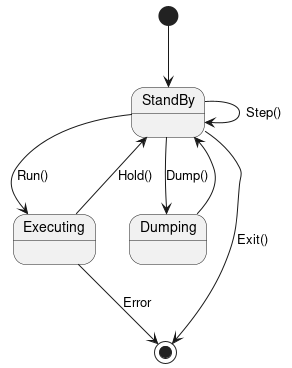
\includegraphics[width=0.35\textwidth]{./Figuras/States.png}
  \caption{Diagrama de estados tentativo del Scheduler.}
  \label{fig:Scheduler}
\end{figure}

\vspace{25px}


\subsection{CPU}

El componente \texttt{CPU} es el encargado de modelar el microprocesador. Será quien interactue con el resto de componentes, siendo el que contiene la lógica de la emulación de cada una de las instrucciones del microprocesador. Entre sus responsabilidades se encuentran:

\begin{itemize}
\item Inicializar los componentes \texttt{MemoryModel}, \texttt{Registers}, \texttt{TimeKeeper} y \texttt{Scheduler}.
\item Cargar el binario a ejecutar en la memoria.
\item Controlar las pausas y reinicios de la emulación.
\end{itemize}


\subsection{C-API}

El componente \texttt{C-API} es el encargado de exponer una API para que el usuario pueda interactuar con el sistema. Dicha API será expuesta mediante una librería dinámica, que podrá ser utilizada desde el lenguage de programación \texttt{C} y \texttt{C++}. Todas las interacciones con el sistema se realizarán a través de esta API.

\end{document}
